\documentclass[a4paper,fleqn,usenatbib]{mnras}

\usepackage{ae, aecompl, amsmath, amssymb}
\usepackage{bm}           %%  bold math
\usepackage{cancel, mathptmx}
\usepackage{color}
\usepackage{dcolumn}  %%  Align table columns on decimal point
\usepackage{epsfig, epsf, etoolbox}
\usepackage{fancyhdr}
\usepackage{graphicx}
\usepackage[T1]{fontenc}
%\usepackage{lscape}
\usepackage{ifthen}
\usepackage{hyperref}
\usepackage{listings}
\usepackage{longtable}
\usepackage{multirow}
\usepackage{newtxtext, newtxmath}
\usepackage{pifont}% http://ctan.org/pkg/pifont
\usepackage{subfigure}
\usepackage{tabu}

\usepackage{verbatim}

\usepackage{xcolor}
%\usepackage[square, sort, comma, numbers]{natbib}
\usepackage{threeparttable}
%\usepackage[square,sort,comma,numbers]{natbib}

\usepackage{graphicx}	% Including figure files
\usepackage{tikz}
\def\checkmark{\tikz\fill[scale=0.4](0,.35) -- (.25,0) -- (1,.7) -- (.25,.15) -- cycle;} 

%%  I dont know why, but arydshln leads to pdflatex crashing (when using 'regular' hline)
%% if you load this package at the top of this list.  e.g. 
%%    tex.stackexchange.com/questions/419497/hline-doesnt-compile-arydshln-and-tabularx-incompatibility
\usepackage{arydshln}


%%%%%%%%%%%%%%%%%%%%%%%%%%%%%%%%%%%%%%%%%%%
%       define Journal abbreviations      %
%%%%%%%%%%%%%%%%%%%%%%%%%%%%%%%%%%%%%%%%%%%
\def\nat{Nat} \def\apjl{ApJ~Lett.} \def\apj{ApJ}
\def\apjs{ApJS} \def\aj{AJ} \def\mnras{MNRAS}
\def\prd{Phys.~Rev.~D} \def\prl{Phys.~Rev.~Lett.}
\def\plb{Phys.~Lett.~B} \def\jhep{JHEP}
\def\npbps{NUC.~Phys.~B~Proc.~Suppl.} \def\prep{Phys.~Rep.}
\def\pasp{PASP} \def\aap{Astron.~\&~Astrophys.} \def\araa{ARA\&A}
\def\jcap{\ref@jnl{J. Cosmology Astropart. Phys.}} 
\def\nar{New~A.R.} 

\newcommand{\preep}[1]{{\tt #1} }

%%%%%%%%%%%%%%%%%%%%%%%%%%%%%%%%%%%%%%%%%%%%%%%%%%%%%
%              define symbols                       %
%%%%%%%%%%%%%%%%%%%%%%%%%%%%%%%%%%%%%%%%%%%%%%%%%%%%%
\def \Mpc {~{\rm Mpc} }
\def \Om {\Omega_0}
\def \Omb {\Omega_{\rm b}}
\def \Omcdm {\Omega_{\rm CDM}}
\def \Omlam {\Omega_{\Lambda}}
\def \Omm {\Omega_{\rm m}}
\def \ho {H_0}
\def \qo {q_0}
\def \lo {\lambda_0}
\def \kms {{\rm ~km~s}^{-1}}
\def \kmsmpc {{\rm ~km~s}^{-1}~{\rm Mpc}^{-1}}
\def \hmpc{~\;h^{-1}~{\rm Mpc}} 
\def \hkpc{\;h^{-1}{\rm kpc}} 
\def \hmpcb{h^{-1}{\rm Mpc}}
\def \dif {{\rm d}}
\def \mlim {m_{\rm l}}
\def \bj {b_{\rm J}}
\def \mb {M_{\rm b_{\rm J}}}
\def \mg {M_{\rm g}}
\def \mi {M_{\rm i}}
\def \qso {_{\rm QSO}}
\def \lrg {_{\rm LRG}}
\def \gal {_{\rm gal}}
\def \xibar {\bar{\xi}}
\def \xis{\xi(s)}
\def \xisp{\xi(\sigma, \pi)}
\def \Xisig{\Xi(\sigma)}
\def \xir{\xi(r)}
\def \max {_{\rm max}}
\def \gsim { \lower .75ex \hbox{$\sim$} \llap{\raise .27ex \hbox{$>$}} }
\def \lsim { \lower .75ex \hbox{$\sim$} \llap{\raise .27ex \hbox{$<$}} }
\def \deg {^{\circ}}
%\def \sqdeg {\rm deg^{-2}}
\def \deltac {\delta_{\rm c}}
\def \mmin {M_{\rm min}}
\def \mbh  {M_{\rm BH}}
\def \mdh  {M_{\rm DH}}
\def \msun {M_{\odot}}
\def \z {_{\rm z}}
\def \edd {_{\rm Edd}}
\def \lin {_{\rm lin}}
\def \nonlin {_{\rm non-lin}}
\def \wrms {\langle w_{\rm z}^2\rangle^{1/2}}
\def \dc {\delta_{\rm c}}
\def \wp {w_{p}(\sigma)}
\def \PwrSp {\mathcal{P}(k)}
\def \DelSq {$\Delta^{2}(k)$}
\def \WMAP {{\it WMAP \,}}
\def \cobe {{\it COBE }}
\def \COBE {{\it COBE \;}}
\def \HST  {{\it HST \,\,}}
\def \Spitzer  {{\it Spitzer \,}}
\def \ATLAS {VST-AA$\Omega$ {\it ATLAS} }
\def \BEST   {{\tt best} }
\def \TARGET {{\tt target} }
\def \TQSO   {{\tt TARGET\_QSO}}
\def \HIZ    {{\tt TARGET\_HIZ}}
\def \FIRST  {{\tt TARGET\_FIRST}}
\def \zc {z_{\rm c}}
\def \zcz {z_{\rm c,0}}


\newcommand{\sqdeg}{deg$^{-2}$}
\newcommand{\lya}{Ly$\alpha$\ }
%\newcommand{\lya}{Ly\,$\alpha$\ }
\newcommand{\lyaf}{Ly\,$\alpha$\ forest}
%\newcommand{\eg}{e.g.~}
%\newcommand{\etal}{et~al.~}
\newcommand{\cii}{C\,{\sc ii}\ }
\newcommand{\ciii}{C\,{\sc iii}]\ }
\newcommand{\civ}{C\,{\sc iv}}
\newcommand{\siiv}{Si\,{\sc iv}\ }
\newcommand{\mgii}{Mg\,{\sc ii}\ }
\newcommand{\feii}{Fe\,{\sc ii}\ }
\newcommand{\feiii}{Fe\,{\sc iii}\ }
\newcommand{\caii}{Ca\,{\sc ii}\ }
\newcommand{\halpha}{H\,$\alpha$\ }
\newcommand{\hbeta}{H\,$\beta$\ }
\newcommand{\oi}{[O\,{\sc i}]\ }
\newcommand{\oii}{[O\,{\sc ii}]\ }
\newcommand{\oiii}{[O\,{\sc iii}]\ }
\newcommand{\heii}{[He\,{\sc ii}]\ }
\newcommand{\nii}{N\,{\sc ii}\ }
\newcommand{\nv}{N\,{\sc v}\ }

%% From:: /cos_pc19a_npr/LaTeX/proposals/JWST/JWST_ERS/Proposal/lines.tex
%%  
\newcommand{\imw}{$i$--$W3$}
\newcommand{\imwf}{$i$--$W4$}
\newcommand{\rmwf}{$r$--$W4$}
\newcommand{\imwt}{$i$--$W2$}
\newcommand{\wtmwf}{$W3$--$W4$}
%\newcommand{\kms}{km s$^{-1}$}
\newcommand{\cmN}{cm$^{-2}$}
\newcommand{\cmn}{cm$^{-3}$}
%\newcommand{\msun}{M$_{\odot}$}
\newcommand{\lsun}{L$_{\odot}$}
\newcommand{\lam}{$\lambda$}
\newcommand{\mum}{$\mu$m}
\newcommand{\ebv}{$E(B$$-$$V)$}
%\newcommand{\heii}{\mbox{He\,{\sc ii}}}
\newcommand{\cv}{\mbox{C\,{\sc v}}}
%\newcommand{\civ}{\mbox{C\,{\sc iv}}}
%\newcommand{\ciii}{\mbox{C\,{\sc iii}}}
%\newcommand{\cii}{\mbox{C\,{\sc ii}}}
%\newcommand{\nv}{\mbox{N\,{\sc v}}}
\newcommand{\niv}{\mbox{N\,{\sc iv}}}
\newcommand{\niii}{\mbox{N\,{\sc iii}}}
%\newcommand{\oi}{\mbox{O\,{\sc i}}}
%\newcommand{\oii}{\mbox{O\,{\sc ii}}}
%\newcommand{\oiii}{\mbox{[O\,{\sc iii}]}}
\newcommand{\oiv}{\mbox{O\,{\sc iv}}}
\newcommand{\ov}{\mbox{O\,{\sc v}}}
\newcommand{\ovi}{\mbox{O\,{\sc vi}}}
\newcommand{\ovii}{\mbox{O\,{\sc vii}}}

%\newcommand{\feii}{\mbox{Fe\,{\sc ii}}}
%\newcommand{\feiii}{\mbox{Fe\,{\sc iii}}}
%\newcommand{\mgii}{\mbox{Mg\,{\sc ii}}}
\newcommand{\neii}{[Ne\,{\sc ii}]\ }
\newcommand{\neiii}{[Ne\,{\sc ii}]\ }
\newcommand{\nev}{Ne\,{\sc v}\ }
\newcommand{\nevi}{[Ne\,{\sc vi}]\ }
\newcommand{\neviii}{\mbox{Ne\,{\sc viii}}}
\newcommand{\aliii}{\mbox{Al\,{\sc iii}}}
\newcommand{\siii}{\mbox{Si\,{\sc ii}}}
\newcommand{\siiii}{\mbox{Si\,{\sc iii}}}
%\newcommand{\siiv}{\mbox{Si\,{\sc iv}}}
%\newcommand{\lya}{\mbox{Ly$\alpha$}}
%\newcommand{\lyb}{\mbox{Ly$\beta$}}
\newcommand{\hi}{\mbox{H\,{\sc i}}}
\newcommand{\snine}{\mbox{[S\,{\sc ix}]}}
\newcommand{\sivi}{\mbox{[Si\,{\sc vi}]}}
\newcommand{\sivii}{\mbox[{Si\,{\sc vii}]}}
\newcommand{\siix}{\mbox{[Si\,{\sc ix}]}}
\newcommand{\six}{\mbox{[Si\,{\sc x}]}}
\newcommand{\sixi}{\mbox{[Si\,{\sc xi}]}}
\newcommand{\caviii}{\mbox{[Ca\,{\sc viii}]}}
\newcommand{\arii}{\mbox{[Ar\,{\sc ii}]}}

%%[Ar II] 6.97
%% [S IX] 1.252 μm 328 
% [Si X] 1.430 μm 351 
% [Si XI] 1.932 μm 401 
% [Si VI] 1.962 μm 167 
% [Ca VIII] 2.321 μm 128 
% [Si VII] 2.483 μm 205 
% [Si IX] 3.935 μm 303
% [Ar II] 6.97


%\snine\ at 1.252$\mu$m, \six\ at 1.430$\mu$m, \sixi\ at 1.932$\mu$m, \sivi\ at
%1.962$\mu$m, \caviii\ at 2.321$\mu$m, \sivi\ at 2.483$\mu$m \siix\ at
%3.935$\mu$m and \arii\ at 6.97$\mu$m. 
%%
%% such as [Ne ii]12.8 μm, [Ne v]14.3 μm, [Ne iii]15.5 μm, [S iii]18.7 μm and 33.48 μm, [O iv]25.89 μm and [Si ii]34.8 μm (e.g
%%
%% MIR emission lines like [NeII] and [NeV] are ..
%%
%% Also,  arXiv:astro-ph/0003457v1 
%% [NeV] 14.32um & 24.32um and [NeVI] 7.65um imply an A(V)>160 towards the NLR...
%% [NeIII]15.56um/[NeII]12.81um
%%
%% [Ne V] 14.3, 24.2 μm 97.
%% [Ne II] 12.8 μm
%% [OIV] 26μm
%%


%%%%%%%%%%%%%%%%%%%%%%%%%%%%%%%%%%%%%%%%%%%%%%%%%%%%%
%              define Listings                       %
%%%%%%%%%%%%%%%%%%%%%%%%%%%%%%%%%%%%%%%%%%%%%%%%%%%%%
\definecolor{dkgreen}{rgb}{0,0.6,0}
\definecolor{gray}{rgb}{0.5,0.5,0.5}
\definecolor{mauve}{rgb}{0.58,0,0.82}

\lstset{frame=tb,
  language=Python,
  aboveskip=3mm,
  belowskip=3mm,
  showstringspaces=false,
  columns=flexible,
  basicstyle={\small\ttfamily},
  numbers=none,
  numberstyle=\tiny\color{gray},
  keywordstyle=\color{blue},
  commentstyle=\color{dkgreen},
  stringstyle=\color{mauve},
  breaklines=true,
  breakatwhitespace=true,
  tabsize=3
}



\title[High-redshift CLQs]{The first high-redshift Changing Look Quasars}

\author[Bercow]
{The RH John~S.~Bercow, MP, {\it et al.} 
%Nicholas~P.~Ross$^{1}$\thanks{E-mail: npross@roe.ac.uk},    
%K. E. Saavik Ford$^{2,3,4}$,  Matthew Graham$^{5}$,  Barry McKernan$^{2,3,4}$,  
%\newauthor Daniel Stern$^{6}$, 
%Aaron M. Meisner$^{7,8}$, Roberto J. Assef$^{9}$, Arjun Dey$^{10}$, Andrew J. Drake$^{11}$, \newauthor Hyunsung D. Jun$^{12}$, Dustin Lang$^{13,14,15}
\\
% List of institutions
$^{1}$Speaker's Chair, The House of Commons, London, SW1A 0AA \\
%$^{1}$Institute for Astronomy, University of Edinburgh, Royal Observatory, Blackford Hill, Edinburgh EH9 3HJ, United Kingdom \\
%$^{2}$Department of Science, BMCC, City University of New York, New York, NY 10007, USA \\
%$^{3}$Department of Astrophysics, Rose Center for Earth and Space, American Museum of Natural History, Central Park West at 79th Street, NY 10024, USA \\
%$^{4}$Graduate Center, City University of New York, 365 5th Avenue, New York, NY 10016, USA\\
%$^{5}$Cahill Center for Astronomy and Astrophysics, California Institute of Technology, Mail Code 249/17, 1200 E California Blvd, Pasadena CA 91125, USA\\
%$^{6}$Jet Propulsion Laboratory, California Institute of Technology, 4800 Oak Grove Drive, Mail Stop 169-221, Pasadena, CA 91109, USA \\
}

\date{Accepted XXX. Received YYY; in original form ZZZ}
\pubyear{2018}

%\hypersetup{draft}
\begin{document}
\label{firstpage}
\pagerange{\pageref{firstpage}--\pageref{lastpage}}
\maketitle


\begin{abstract}
Lorem ipsum dolor sit amet, consectetur adipiscing elit. Nunc imperdiet facilisis volutpat. Phasellus ultricies justo a ante bibendum porta. Nulla varius convallis risus in tincidunt. Vivamus sit amet massa non dui volutpat porttitor. Donec imperdiet mauris non risus commodo tempor. Nulla volutpat nulla a lorem lobortis, a luctus nulla rhoncus. Vestibulum vel ante elementum nisl feugiat sollicitudin. Aenean purus sem, mattis vitae odio et, varius vehicula nulla.
%%
Nulla ante mauris, mattis a tristique eu, pharetra eget erat. Cras et ultrices lectus. Praesent augue erat, commodo ac malesuada vel, mattis ac nisi. Quisque eu vehicula urna, in fringilla nunc. Duis faucibus scelerisque felis, sollicitudin luctus tortor pretium dapibus. Sed cursus scelerisque dapibus. Proin a bibendum neque, sit amet aliquet arcu. Vivamus in eros lectus. Nam dui felis, convallis sit amet dolor ut, dignissim posuere nunc. Donec egestas tellus vel urna interdum tincidunt. Sed orci eros, convallis in rhoncus sit amet, tincidunt ac est. Mauris tempus, diam a euismod tempus, est turpis laoreet justo, quis posuere augue ipsum sed nisi. Aliquam non lobortis tellus. Morbi vulputate porta placerat. Quisque dapibus pretium arcu eget tempor. Aenean in tincidunt nisi. Aenean interdum congue enim.
\end{abstract}

% Select between one and six entries from the list of approved keywords.
% Don't make up new ones.
\begin{keywords}
accretion, accretion discs -- surveys -- quasars: general -- quasars: individual: J1100-0053 
\end{keywords}



%%%%%%%%%%%%%%%%%%%%%%%%%%%%%%%%%%%%%%%%%%%%%%%%%%%%%%%%%%%%%%%%%%%%%%%%%%%%%%%%%
%%%%%%%%%%%%%%%%%%%%%%%%%%%%%%%%%%%%%%%%%%%%%%%%%%%%%%%%%%%%%%%%%%%%%%%%%%%%%%%%%
%%
%%
%%   SECTION 1  SECTION 1  SECTION 1  SECTION 1  SECTION 1  SECTION 1  
%%   SECTION 1  SECTION 1  SECTION 1  SECTION 1  SECTION 1  SECTION 1  
%%   SECTION 1  SECTION 1  SECTION 1  SECTION 1  SECTION 1  SECTION 1  
%%
%%
%%%%%%%%%%%%%%%%%%%%%%%%%%%%%%%%%%%%%%%%%%%%%%%%%%%%%%%%%%%%%%%%%%%%%%%%%%%%%%%%%%
%%%%%%%%%%%%%%%%%%%%%%%%%%%%%%%%%%%%%%%%%%%%%%%%%%%%%%%%%%%%%%%%%%%%%%%%%%%%%%%%%%
\section{Introduction}
Luminous AGN, i.e. quasars, are now seen to significantly vary their energy output on timescales of weeks to months. 
This observational fact, and the subsequent mismatch in the expected timescale, the ``viscous'' timescale, 
which for a $\approx$10$^{7}$ M$_{\odot}$ is $\sim$hundreds of years, was noted over 30 years ago \citep[e.g.][]{Alloin1985}. 
However, with new photometric light-curve and repeat spectroscopic data, the desire for a deeper understanding 
of AGN accretion disk physics  has been re-established \citep[e.g.][]{Lawrence2018, Antonucci2018}. 

Samples of over 100 ``Changing Look'' quasars (CLQs) or ``Changing State'' quasars (CSQs) have now been 
assembled \citep[e.g.][]{MacLeod2019, Graham2019}. The community uses both these
terms as a cover for the underlying physics. For sake of argument, ``Changing Look'' quasars can be 
thought of as the extension of ``regular'' quasar variability \citep[e.g.][]{MacLeod2012} whereas 
the ``Changing State'' quasars (CSQs) have a `state-transition' similar to that in Galactic X-ray binaries
\citep[e.g][]{NodaDone2018, Ruan2019}. 

While there have been a slew of studies on triply ionized carbon, i.e \civ, broad absorption line quasars
\citep[BAL QSOs; see e.g. Table 1][]{Hemler2019}, dramatic changes in the 
broad {\it emission} line (BEL) of \civ, and indeed, \ciii have not to this point been seen. 
%% 
Here, we report on three objects 
SDSS J120544.7+342252.4  (hereafter J1205+3422), 
SDSS J163852.93+282707.7 (hereafter J1638+2827) and
SDSS J222818.76+220102.9 (hereafter J2228+2201)  
which show dramatic changes in the \civ broad emission line
properties, as well as in the underlying continuum. We claim these are
the first examples of ``Changing Look Quasars'' at high ($z>1$)
redshift and for emission lines with high ionization potentials
(I.P.'s $>$13.6 eV).

For J1638+2827, over the course of 1279 days observed, 400 days in the rest-frame, the  broad \civ and \ciii BEL start to fade.  
For J2228+2201, over the course of 771 days observed, 240 days in the rest-frame, broad \civ and \ciii BELs both emerge and the 
standard UV/blue continuum slope increases in flux. 
the UV/blue continuum diminishes and the shape of \lya changes. 


\subsection{Literature Search}
\citet{Wilhite2006} examine the variability of the high-ionizaton
C~\textsc{iv}$\lambda{1549}$ line in a sample of 105 quasars observed
at multiple epochs by the Sloan Digital Sky Survey.  We find a strong
correlation between the change in the C~\textsc{iv} line flux and the
change in the line width, but no correlations between the change in
flux and changes in line center and skewness.  The relation between
line flux change and line width change is consistent with a model in
which a broad line base varies with greater amplitude than the line
core. The objects studied here are more luminous and at higher
redshift than those normally studied for variability, ranging in
redshift from 1.65 to 4.00 and in absolute $r$-band magnitude from
roughly $-$24 to $-$28.  Using moment analysis line-fitting
techniques, we measure line fluxes, centers, widths and skewnesses for
the C~\textsc{iv} line at two epochs for each object.  The well-known
Baldwin Effect is seen for these objects, with a slope $\beta =
-0.22$.  The sample has a median intrinsic Baldwin Effect slope of
$\beta_{int} = -0.85$; the C~\textsc{iv} lines in these
high-luminosity quasars appear to be less responsive to continuum
variations than those in lower luminosity AGN.  Additionally, we find
no evidence for variability of the well known blueshift of the
C~\textsc{iv} line with respect to the low-ionization
Mg~\textsc{ii}$\lambda$2798 line in the highest flux objects,
indicating that this blueshift might be useful as a measure of
orientation.


%% NAZAROVA 2003
%% BROAD EMISSION LINES La, C IV AND Hb IN NGC 5548
%% Astronomical and Astrophysical Transactions
%% Vol. 22, Nos. 4–5, August–October 2003, pp. 681–689

%% Punsly 2010
%% Astrophysical Journal, 713, 232
%% THE REDSHIFTED EXCESS IN QUASAR C iv BROAD EMISSION LINES


Denney, Klly; SDSS-RM Team \\
The Effects of S/N on Measuring CIV Broad Emission Line Widths in Quasars - An Early Science Result from the Sloan Digital Sky Survey Reverberation Mapping Project\\
http://adsabs.harvard.edu/abs/2015AAS...22520403D\\

%% Coatman et al. (2017, AAS; http://adsabs.harvard.edu/abs/2017AAS...22930203C) 
%%Accurate black-hole (BH) mass estimates for high-redshift (z>2) quasars are essential for better understanding the relationship between super-massive BH accretion and star formation. Progress is currently limited by the large systematic errors in virial BH-masses derived from the CIV broad emission line, which is often significantly blueshifted relative to systemic, most likely due to outflowing gas in the quasar broad-line region. We have assembled Balmer-line based BHmasses for a large sample of 230 high-luminosity (1045.5-1048 ergs-1), redshift 1.5<z<4 quasars, which, for the first time, span the entire range of CIV blueshifts seen in the quasar population. We find the CIV-based BH-masses to be larger than the corresponding Balmer line-based masses by almost an order of magnitude at the most extreme blueshifts (˜5000 kms-1). An empirical correction to the CIV BH-masses is derived, which depends only on the properties of the CIV line itself (i.e. blueshift and FWHM). 
%%
\citet{Coatman2017AAS} show that this new correction now enables the derivation of un-biased CIV-based virial BH masses for the majority of high-luminosity, high-redshift quasars.In the same high-luminosity quasar sample, we find the narrow [OIII] emission to be weaker and more asymmetric than is generally found in  lower-luminosity AGN and that a significant fraction of our quasars have exceptionally broad (FWHM $> 3000 km s^{-1}$), blueshifted [OIII] emission. We find a strong correlation between the \civ and [OIII] blueshifts. This correlation holds even for quasars at fixed
luminosity and suggests that broad line region outflows in quasars are
connected to galaxy-scale winds.

%% \citet{Coatman2017} 
The \civ $\lambda \lambda$1498,1501 broad emission line is visible in optical spectra to redshifts exceeding $z\sim5$. \civ has long been known to exhibit significant displacements to the blue and these `blueshifts' almost certainly signal the presence of strong outflows. As a consequence, single-epoch virial black hole (BH) mass estimates derived from \civ velocity widths are known to be systematically biased compared to masses from the hydrogen Balmer lines. 
\citet{Coatman2017} use a large sample of 230 high-luminosity (LBol = 1045.5-1048 erg s-1), redshift $1.5 < z < 4.0$ quasars with both \civ and Balmer line spectra, we have quantified the bias in \civ BH masses as a function of the \civ blueshift. \civ BH masses are shown to be a factor of 5 larger than the corresponding Balmer-line masses at C IV blueshifts of 3000 km s-1 and are overestimated by almost an order of magnitude at the most extreme blueshifts, $\gtrsim$5000 km s$^{-1}$. Using the monotonically increasing relationship between the \civ blueshift and the mass ratio BH(\civ)/BH(H$\alpha$), we derive an empirical correction to all C IV BH masses. The scatter between the corrected C IV masses and the Balmer masses is 0.24 dex at low C IV blueshifts ($\sim$0 km s-1) and just 0.10 dex at high blueshifts ($\sim$3000 km s$^{-1}$), compared to 0.40 dex before the correction. The correction depends only on the C IV line properties - i.e. full width at half-maximum and blueshift - and can therefore be applied to all quasars where C IV emission line properties have been measured, enabling the derivation of unbiased virial BH-mass estimates for the majority of high-luminosity, high-redshift, spectroscopically confirmed quasars in the literature.

\citet{Sun2018} use the multi-epoch spectra of 362 quasars from the Sloan Digital Sky Survey Reverberation Mapping project to investigate the dependence of the blueshift of \civ relative to \mgii on quasar properties. We confirm that high-blueshift sources tend to have low \civ equivalent widths (EWs), and that the low-EW sources span a range of blueshift. Other high-ionization lines, such as He II, also show similar blueshift properties. The ratio of the line width (measured as both the full width at half maximum and the velocity dispersion) of \civ to that of \mgii increases with blueshift. Quasar variability enhances the connection between the \civ blueshift and quasar properties (e.g., EW). The variability of the \mgii line center (i.e., the wavelength that bisects the cumulative line flux) increases with blueshift. In contrast, the C IV line center shows weaker variability at the extreme blueshifts. Quasars with the high-blueshift \civ lines tend to have less variable continuum emission, when controlling for EW, luminosity, and redshift. Our results support the scenario that high-blueshift sources tend to have large Eddington ratios.

%% Romain A. Meyer, Sarah E. I. Bosman, Richard S. Ellis  https://arxiv.org/abs/1902.04558v1
\citet{Meyer2019} present the results of a model-independent investigation of the rest-frame UV spectra from a comprehensive sample of 394 quasars in the redshift range $1.5\leq z \leq 7.5$. We fit the main Broad Emission Lines (BELs) in the rest-frame range 1280 \AA $\leq \lambda \leq $3000 \AA (O I, C II, Si IV, C III, C IV and Mg II) with a lightly-supervised spline fitting technique. Redshifts are derived from the peaks of each fitted BEL and used to compute relative velocity shifts. We show that our method gives unbiased velocity shifts and is insensitive to spectral resolution and instrumental parameters. It is found that the average blueshift of the \civ\, line with respect to several low-ionisation lines in luminosity-matched samples does not significantly evolve over $1.5\leq z\leq 6$. However, the average blueshift increases significantly by a factor $\sim$2.5 at $z \geq 6$. We propose that this redshift evolution can be explained by \civ\, winds launched perpendicularly to an accretion disk with increased torus opacity at high-redshift, coupled with a potential orientation-driven selection bias. Our results open new exciting avenues of investigation into young quasars in the reionisation epoch.

\citet{Richards2011} 
use a sample of $\sim$30,000 quasars from the 7th Data Release of the Sloan Digital Sky Survey, and explore the range of properties exhibited by high-ionization, broad emission lines, such as \civ $\lambda$1549. Specifically, we investigate the anti-correlation between continuum luminosity and emission-line equivalent width (the Baldwin Effect (BEff)) and the ``blueshifting''of the high-ionization emission lines with respect to low-ionization emission lines. 
%Employing improved redshift determinations from Hewett \& Wild, the blueshift of the C IV emission line is found to be nearly ubiquitous, with a mean shift of ~810 km s-1 for radio-quiet (RQ) quasars and ~360 km s-1 for radio-loud (RL) quasars. The BEff is present in both RQ and RL samples. We consider these phenomena within the context of an accretion disk-wind model that is modulated by the nonlinear correlation between ultraviolet and X-ray continuum luminosity. Composite spectra are constructed as a function of C IV emission-line properties in an attempt to reveal empirical relationships between different line species and the continuum. Within a two-component disk+wind model of the broad emission-line region (BELR), where the wind filters the continuum seen by the disk component, we find that RL quasars are consistent with being dominated by the disk component, while broad absorption line quasars are consistent with being dominated by the wind component. Some RQ objects have emission-line features similar to RL quasars; they may simply have insufficient black hole (BH) spin to form radio jets. Our results suggest that there could be significant systematic errors in the determination of L bol and BH mass that make it difficult to place these findings in a more physical context. 
It is possible to classify quasars in a paradigm where the diversity of BELR parameters is due to differences in an accretion disk wind between quasars (and over time); these differences are underlain primarily by the spectral energy distribution, which ultimately must be tied to BH mass and accretion rate.

%\includegraphics\includegraphics[]{../../../../../Users/npr1/Downloads/Richards_2011_AJ_141_167.pdf}

%\citet{1994}
%\includegraphics[]{../../../../../Users/npr1/Downloads/1994ApJ___425__622P.pdf}

%\citet{1994}
%\includegraphics[]{../../../../../Users/npr1/Downloads/1994ASPC___69____1P.pdf}

\citet{Denney2016}
%\includegraphics[]{../../../../../Users/npr1/Downloads/Denney_2016_ApJS_224_14.pdf}
investigate the dependence on data quality of quasar properties
measured from the C IV emission line region at high redshifts.  Our
measurements come from 32 epochs of Sloan Digital Sky Survey
Reverberation Mapping Project spectroscopic observations of 482 $z >
1.46$ quasars. We compare the differences between measurements made
from the single-epoch (SE) and coadded spectra, focusing on the \civ
$\lambda$1549 emission line because of its importance for studies of
high-redshift quasar demographics and physical properties, including
black hole masses. In addition to statistical errors increasing (by
factors of $\sim2-4$), we find increasing systematic offsets with
decreasing signal-to-noise ratio (S/N).

\citet{Grier2015}....
%\includegraphics[]{../../../../../Users/npr1/Downloads/Grier_2015_ApJ_806_111.pdf}

\citep{Corbin1991, Dimitrijevic1992, Wills1993, Brotherton1994, Osmer1994} ...

\citep{Nazarova2003} ...


%\includegraphics[]{../../../../../Users/npr1/Downloads/Misawa_2007_ApJ_660_152.pdf}
%\includegraphics[]{../../../../../Users/npr1/Downloads/Punsly_2010_ApJ_713_232.pdf}
%\includegraphics[]{../../../../../Users/npr1/Downloads/Sun_2015_ApJ_811_42.pdf}
%\includegraphics[]{../../../../../Users/npr1/Downloads/Joshi_2019_ApJ_871_43.pdf}




\begin{figure}
  \centering
  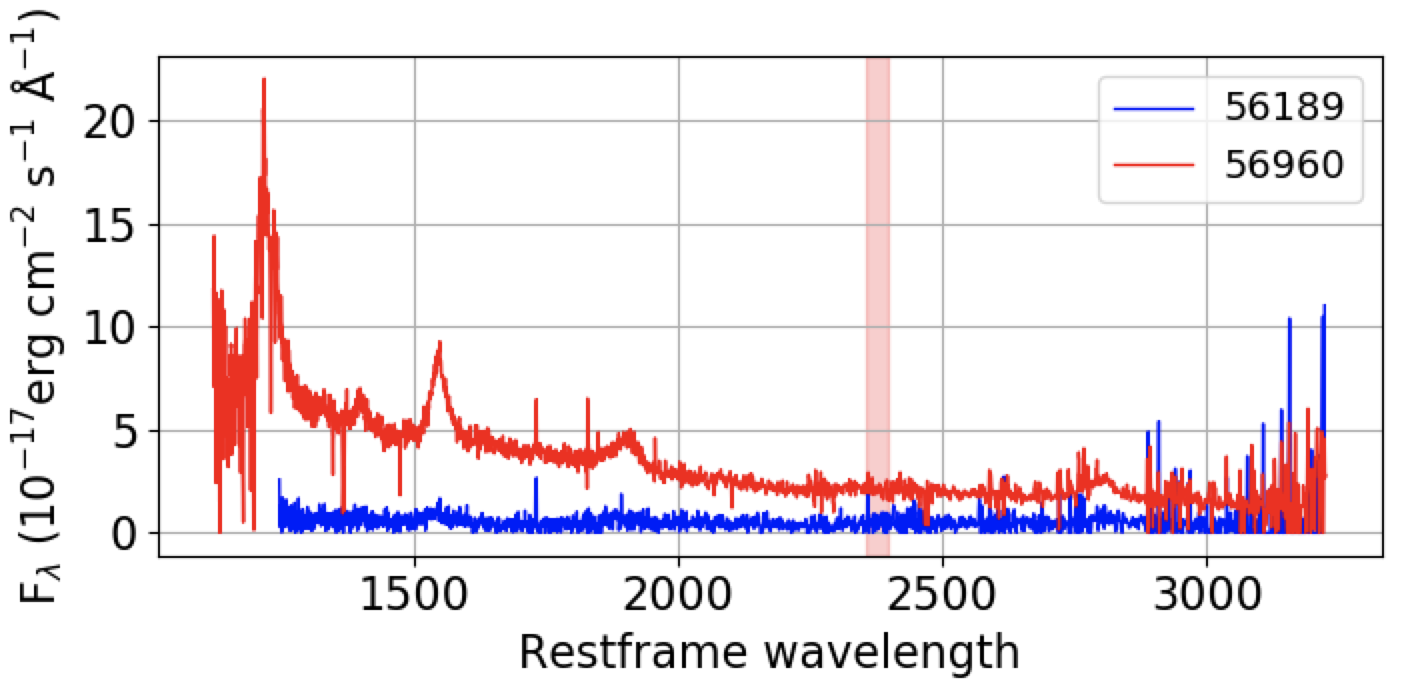
\includegraphics[width=8.7cm, trim=0.2cm 0.2cm 0.2cm 0.2cm, clip]
  {figures/J2228+2201.png}
  \vspace{-12pt}
  \caption[]{J222818.7+220102.6. 
% EMERGING., 
The light curve shows it brightening from 20.5 to 19.5 over the 771 days observed-frame between the two SDSS spectra available. 
A quasar at $z = 2.2$ with the two spectra showing CIV and CIII] emerging on a new blue contiuum slope.}
  \label{fig:disk_suppression}
\end{figure}


\begin{figure}
  \centering
  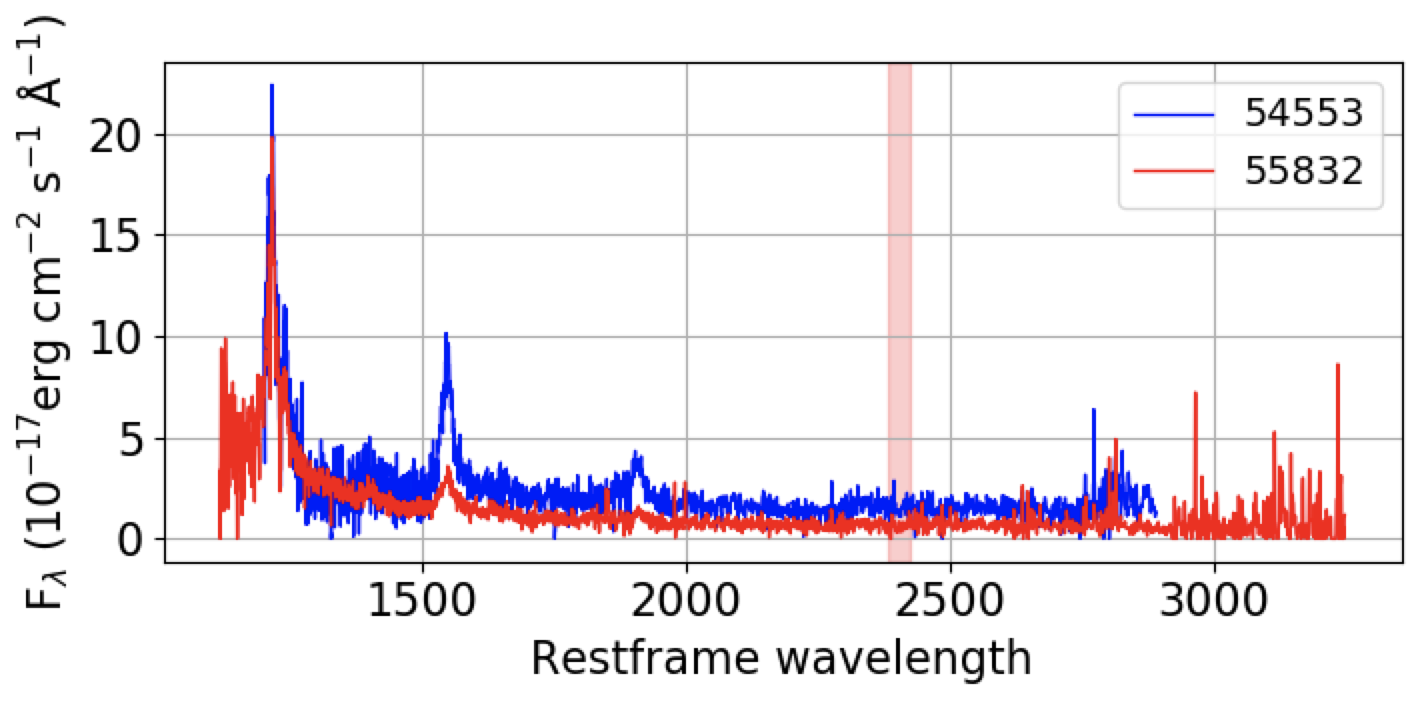
\includegraphics[width=8.7cm, trim=0.2cm 0.2cm 0.2cm 0.2cm, clip]
  {figures/J1638+2827.png}
  \vspace{-12pt}
  \caption[]{The quasar SDSS J163852.9+282708. 
% Disappearing 
A quasar at $z = 2.2$ with the two spectra showing CIV and CIII] fading.}
  \label{fig:disk_suppression}
\end{figure}

%%%%%%%%%%%%%%%%%%%%%%%%%%%%%%%%%%%%%%%%%%%%%%%%%%%%%%%%%%%%%%%%%%%%%%%%%%%%%
%%%%%%%%%%%%%%%%%%%%%%%%%%%%%%%%%%%%%%%%%%%%%%%%%%%%%%%%%%%%%%%%%%%%%%%%%%%%%
%%
%%   SECTION 2   SECTION 2   SECTION 2   SECTION 2   SECTION 2   SECTION 2  
%%   SECTION 2   SECTION 2   SECTION 2   SECTION 2   SECTION 2   SECTION 2  
%%   SECTION 2   SECTION 2   SECTION 2   SECTION 2   SECTION 2   SECTION 2  
%%
%%%%%%%%%%%%%%%%%%%%%%%%%%%%%%%%%%%%%%%%%%%%%%%%%%%%%%%%%%%%%%%%%%%%%%%%%%%%%
%%%%%%%%%%%%%%%%%%%%%%%%%%%%%%%%%%%%%%%%%%%%%%%%%%%%%%%%%%%%%%%%%%%%%%%%%%%%%
\section{Data}
\subsection{Selection/Identification}

\subsection{SDSS spectra}
\begin{table}
 \centering
 \begin{tabular}{l l l l}
  \hline \hline 
% &&\\
   Quantity \ Object                           & J2228+2201     &  J1638+2827 \\
% &&\\
 \hline 
    &&\\
    R.A. / deg                                        &    337.078194      &  249.720559\\
    Declination / deg                            &    +22.017478      &  +28.452159 \\
    redshift, $z$                                    &   2.222$\pm$0.00038   &  2.185$\pm$0.00043          \\
    &&\\ 
    \multirow{2}{*}{Plate, Fiber, MJD}   & 6118, 720, 56189	     &  2948, 614, 54553	  \\
                                         & 7582, 790, 56960	     & 5201, 178, 55832 \\    
 %   &&\\ 
    %$M_{i}(z=2)$  / mag                          &   ?                       & ?                \\
    %log $(L_{\rm bol} / {\rm erg s}^{-1}) $      &   ?             & 45.56$\pm$0.004      & 45.07$\pm$0.004 \\
    %log $(M_{\rm BH} / M_{\odot})  $           &  ?                  & 8.43$\pm$0.03           & 8.46$\pm$0.02 \\
    %Eddington ratio  (\%)                        &  ?                               &  10.7                           &  3.2     \\ 
    &&\\
    \hline \hline 
  \end{tabular}
  \caption{Physical properties of J1100-0053, J2317+0005 and J1052+1519 using the
    methods from \citet{Shen2011}. *This spectrum was used to estimate
    the quantities reported.  We use the regular definition of $L_{\rm
      Edd} = 4 \pi G M m_{\rm p} c /\sigma_{T} =
    1.26\times10^{38}\left (M/M_{\odot} \right )$ erg s$^{-1}$.} 
 \label{tab:Shen_props}
\end{table}

Double Spectrograph (DBSP) is a low-to-medium resolution ($R\sim$1,000
to 10,000) grating instrument for the Palomar 200-inch telescope
Cassegrain focus that uses a dichroic (at, e.g., 5200\AA\ ) to split
light into simultaneously observed separate red and blue channels. 

The Low Resolution Imaging Spectrometer (LRIS) is a visible-wavelength
imaging and spectroscopy instrument commissioned in 1993 and operating
at the Cassegrain focus of 10-meter Keck I telescope. 

\begin{table*}
 \centering
 \begin{tabular}{r  r  r r r   r r r r}
  \hline \hline 
% &&\\
   Object                         & \multirow{3}{*}{Redshift} & \multirow{3}{*}{Mag}      & \multirow{3}{*}{MJD} & \multirow{3}{*}{Date}  & \multirow{3}{*}{Instrument}   & Exposure    & \multirow{3}{*}{Spectrum} & \multirow{3}{*}{Notes} \\
   R.A. / deg                   &               &               &            &                                &                                                                       &  Time         & & \\
   Decl. / deg                 &               &               &            &                                &                                                                       &  / seconds         & & \\

% &&\\
 \hline 
                                       &                &               &            &                              &                   &                             &  & \\
   J120544.7+342252.4   & 2.071     &   17.99   & 53498 & 2005-May-08   & SDSS             & ?                          & 53498-2089-427  & \\
          181.436164           &                &               & 58538 & 2019-Feb-24     & DBSP            &  2$\times$900    &                               &  Conditions? \\
         +34.381229           &                &               & 58693 & 2019-Jul-29      & DBSP            &  2$\times$1200   &                                &   \\
                                       &                &               &              &                           &                   &                             &  & \\
   J163852.9+282707.7   & 2.182     &   19.77    & 54553 & 2008-Mar-28    & SDSS             & ?                          & 54553-2948-614  & \\
      249.720558407	       &               &              & 55832  & 2011-Sep-28     & BOSS            &   3603                  & 55832-5201-178  & \\
       +28.452158884        &               &              & 58583 & 2019-Apr-10        & LRIS              &  2$\times$900    &   & \\
                                       &                &               &              &                           &                   &                             &  & \\
    J222818.7+220102.9   & 2.222     & 19.97    & 56189 & 2012-Sep-19     & BOSS             &  2702               & 56189-6118-720   & \\
        337.078194              &              &              & 56960 & 2014-Oct-30    & BOSS             & ?                         & 56960-7582-790     & QSO1-REOBS \\ 
        +22.017478                                &               &             & 58693 & 2019-Jul-29      & DBSP              & 2$\times$1200  &       &    \\
                                       &                &               &            &                             &                   &                              &  & \\
%   J232446.7+140029.5   &  0.916     &  18.83   &  56209 & 2012-Oct-09   & BOSS             & ?                             & 56209-6148-743   & \\
 %                                      &                &               &   58662 & 2019-Jun-28  &   (??)DBSP       & ?                            &  & \\
  %                                     &                &               &              &                           &                   &                              &  & \\
   \hline \hline   
  \end{tabular}
  \caption{Spectrum is SDSS/BOSS MJD-Plate-FiberID combination. 
Exposure times are from the {\tt plate.fits} file. 
DBSP on the Palomar 200-inch telescope is the } 
 \label{tab:obs_notes}
\end{table*}


\subsection{J1205+3422 }
SDSS J120544.67+342252.4, observed by SDSS, first reported in \citet{Schneider2007}. 
Redshift of $z=$2.068$\pm$0.00027. 
%% targeting_flags	SERENDIP_BLUE QSO_CAP
plate	2089 
mjd	53498
fiberid	427


\subsection{J1638+2827}
SDSS J163852.93+282707.7       16h38m52.9s +28d27m08s  \\
First reported in \citet{Schneider2010}. 
Selected by {\tt SERENDIP\_BLUE} and {\tt QSO\_MAG\_OUTLIER} in SDSS \citep{Richards2002}, meaning...
Selected as a $z>2$ known quasar and passed BOSS quasar target selections \citep{Ross2012}. 


R.A. (J2000) = 249.72058 degs. \\
Decl. (J2000) = 28.45217 degs. \\
\href{skyserver.sdss.org/dr15/en/tools/explore/Summary.aspx?id=1237662301375824232}{SDSS SkyServer} 
All Spectra of this Object:: \\
specObjId	plate	MJD	fiber	ra	dec	redshift \\
5855854441601671168	5201	55832	178	2.186$\pm$0.00073\\
3319321776793610240	2948	54553	614	2.185$\pm$0.00043\\


\subsection{J2228+2201}
SDSS J222818.76+220102.9 (R.A. 337.078194926, Decl. 22.017477924) was first reported in 
\citet{Paris2017}. 

%%\href{https://skyserver.sdss.org/dr12/en/tools/chart/navi.aspx?ra=337.077916666667&dec=22.0173888888889&scale=0.2&width=120&height=120&opt=
\href{skyserver.sdss.org/dr15/en/tools/explore/summary.aspx?id=1237678579819479655}{SDSS SkyServer}
All Spectra of this Object:: \\
specObjId	plate	MJD	fiber	ra	dec	redshift \\
8536790363997708288	7582	56960	790	2.222$\pm$0.00038\\
6888453645991387136	6118	56189	720	2.217$\pm$0.00208\\



%Plate: 2948, MJD: 54553, Fiber: 0614
%https://dr12.sdss.org/spectrumDetail?mjd=54553&fiber=614&plateid=2948

\begin{table*}
  \centering
  \begin{tabular}{l  l  l    lll}
    \hline \hline 
    Line 	    &   Rest	      & Line       & Line	       &	Line			                 &   Continuum \\ 
    Name	    &   Wavelength  &  $z$       & $\sigma$ 	&	Flux			                 & \\
                    &    $\AA $        &              & /  km s$-1$	&     10$^{-17}$ erg/cm$2$/s &  10$^{-17}$ erg/cm$^2$/s/\AA  \\
Ly$\alpha$  &	 1215.7	&	2.186      &	1362	&	510.5		                &	7.224 \\
\nv		    &   1240.8	&	2.184     &	 854.6	&	122.4	                    	&	5.546 \\ 
\civ		    &  1549.5	&	2.184    &	1927	&	462.6		                &	2.722 \\ 
\heii	    &	 1640.4	&	2.184    &	1927	&    	  8.067	                   	&	2.447 \\  
\ciii 	    &	 1908.7	&	2.184    &	1927	&	164.6	                   	&	1.966  \\ 
\mgii	    &	 2800.3	&	2.184   & 	1927	&	187.4	                   	&	1.513  \\
   \hline \hline   
  \end{tabular}
  \caption{Line Measurement Information}
 \label{tab:line_values}
\end{table*}



\begin{table*}
  \centering
  \begin{tabular}{l  lll lll  }
    \hline \hline 
                                    &                               &                                           &                                                      &                                  &                         & \\  
                                  \multicolumn{7}{c}{J1638+2827}  \\
                                    &                               &                                           &                                                      &                                  &                         & \\  
   \hline                       
%                                   &                               &                                           &                                                      &                                  &                         & \\  
    Line      	             & Line  $\sigma$     & Line  Flux                           &   Continuum                                 & Line  $\sigma$          & Line  Flux        &   Continuum                                    \\
%    Wavelength	             & /  km s$^{-1}$         &   10$^{-17}$ erg/cm$2$/s  & 10$^{-17}$ erg/cm$^2$/s/\AA      &  /  km s$-1$             & / 10$^{-17}$ erg/cm$2$/s   & /10$^{-17}$ erg/cm$^2$/s/\AA       \\
                                     & \multicolumn{3}{l}{MJD 54553}                                                                                   & \multicolumn{3}{l}{MJD 55832}                                                                                                          \\
    Ly$\alpha$1215.7    &  1362	            &	510.5		                  &	7.224                                           &  1769	                &   633.9	              &  5.376     \\
    \nv1240.8	            &   854.6	            &	122.4	                    	  &	5.546                                           & 1012	                &  107.1		      &  4.645\\ 
    \civ1549.5         	    &	 1927	            &	462.6		                  &	2.722                                           & 2287	                &  125.1		      &  1.256      \\  
    \heii1640.4	            &	 1927    	            &      8.067	                   	  &	2.447                                           & 2287	                &    10.68	      &  1.001\\  
    \ciii1908.7        	    &	 1927	            &	164.6	                   	  &	1.966                                          & 2287	 	                &     29.53	      &  0.6008\\ 
    \mgii2800.3	    &   1927	            &	187.4	                   	  &	1.513                                          & 2287 	 	         &    34.66	      &  0.3461  \\
                                    &                               &                                           &                                                      &                                  &                           &                \\  
   \hline \hline   
  \end{tabular}
  \caption{Line Measurement Information. 
    Line $\sigma$ in units of   km s$-1$; 
    Line flux          in units of  10$^{-17}$ erg/cm$^2$/s; 
    Continuum      in units of  10$^{-17}$ erg/cm$^2$/s/ \AA; 
}
 \label{tab:line_values}
\end{table*}


%Plate: 5201, MJD: 55832, Fiber: 178
%https://dr12.sdss.org/spectrumDetail?mjd=55832&fiber=178&plateid=5201

%Line		Rest		        Line	        Line		        Line			   Continuum
%Name		Wavelength	z	        sigma 		Flux	
%                       [Å]			               [km s-1]  	[10-17erg/cm2/s] 	   [10-17erg/cm2/s/Å]
%Ly_alpha	1215.7		2.186	1769		633.9		   5.376
%N_V		1240.8		2.185	1012		107.1		   4.645
%C_IV		1549.5		2.185	2287		125.1		   1.256
%He_II		1640.4		2.185	2287		 10.68		   1.001
%C_III]		1908.7		2.185	2287	 	 29.53		   0.6008
%Mg_II		2800.3		2.185	2287 	 	 34.66		   0.3461

%So, ratios, MJD 54553 / MJD 55832::
%$Ly_alpha	1215.7		—	0.770		0.805			1.344			
%N_V		1240.8		—	0.844		1.143			1.194
%C_IV		1549.5		—	0.843		3.698			2.167			
%He_II		1640.4		—	0.843		0.755			2.445			
%C_III]		1908.7		—	0.843		5.574			3.27			
%Mg_II		2800.3		—	0.843		5.407			4.37





\subsection{Multi-wavelength properties}
MIR \\
Radio \\



%%%%%%%%%%%%%%%%%%%%%%%%%%%%%%%%%%%%%%%%%%%%%%%%%%%%%%%%%%%%%%%%%%%%%%%%%%%%%
%%%%%%%%%%%%%%%%%%%%%%%%%%%%%%%%%%%%%%%%%%%%%%%%%%%%%%%%%%%%%%%%%%%%%%%%%%%%%
%%
%%   SECTION 3   SECTION 3   SECTION 3   SECTION 3   SECTION 3   SECTION 3  
%%   SECTION 3   SECTION 3   SECTION 3   SECTION 3   SECTION 3   SECTION 3  
%%   SECTION 3   SECTION 3   SECTION 3   SECTION 3   SECTION 3   SECTION 3  
%%
%%%%%%%%%%%%%%%%%%%%%%%%%%%%%%%%%%%%%%%%%%%%%%%%%%%%%%%%%%%%%%%%%%%%%%%%%%%%%
%%%%%%%%%%%%%%%%%%%%%%%%%%%%%%%%%%%%%%%%%%%%%%%%%%%%%%%%%%%%%%%%%%%%%%%%%%%%%
\section{Results}
\subsection{In the context of CLQs at lower-$z$}

\subsection{Balmer CLQs vs. \civ CLQs}


%%%%%%%%%%%%%%%%%%%%%%%%%%%%%%%%%%%%%%%%%%%%%%%%%%%%%%%%%%%%%%%%%%%%%%%%%%%%%
%%%%%%%%%%%%%%%%%%%%%%%%%%%%%%%%%%%%%%%%%%%%%%%%%%%%%%%%%%%%%%%%%%%%%%%%%%%%%
%%
%%   SECTION 4   SECTION 4   SECTION 4   SECTION 4   SECTION 4   SECTION 4  
%%   SECTION 4   SECTION 4   SECTION 4   SECTION 4   SECTION 4   SECTION 4  
%%   SECTION 4   SECTION 4   SECTION 4   SECTION 4   SECTION 4   SECTION 4  
%%
%%%%%%%%%%%%%%%%%%%%%%%%%%%%%%%%%%%%%%%%%%%%%%%%%%%%%%%%%%%%%%%%%%%%%%%%%%%%%
%%%%%%%%%%%%%%%%%%%%%%%%%%%%%%%%%%%%%%%%%%%%%%%%%%%%%%%%%%%%%%%%%%%%%%%%%%%%%
\section{Discussion and Conclusions}


\bibliographystyle{mnras}
\bibliography{tester_mnras}


% Don't change these lines
\bsp	% typesetting comment
\label{lastpage}
\end{document}


\end{document}